\chapter{Implémentation, Tests et Résultats}

\section{Introduction}

Ce chapitre présente l'implémentation concrète de SmartClub Analytics, les tests effectués, et les résultats obtenus. Nous détaillons les aspects techniques du développement, les choix d'implémentation, et les performances du système.

\section{Environnement de Développement}

\subsection{Stack Technique}

\begin{table}[H]
\centering
\begin{tabular}{|l|l|l|}
\hline
\textbf{Couche} & \textbf{Technologie} & \textbf{Version} \\
\hline
Backend & Python / Django & 5.1.4 / 5.1 \\
API REST & Django REST Framework & 3.15 \\
Base de données & PostgreSQL & 16 \\
Frontend & React & 18 \\
CSS & Tailwind CSS & 3.4 \\
Visualisation & Recharts & 2.12 \\
LLM & Groq API (Llama 3.1 8B) & 2025-04 \\
ML & Scikit-learn & 1.6 \\
Conteneurisation & Docker / Docker Compose & 27 \\
\hline
\end{tabular}
\caption{Technologies utilisées dans SmartClub Analytics}
\label{tab:tech-stack}
\end{table}

\subsection{Structure du Projet}

\begin{lstlisting}[style=codeframe]
SmartClub_Analytics/
├── backend/
│   ├── smartclub/           # Projet Django principal
│   ├── physio/              # Module physiothérapie
│   │   ├── models.py        # Modèles de données
│   │   ├── views.py         # Endpoints REST API
│   │   ├── views_v2.py      # Version 2 améliorée
│   │   ├── serializers.py   # Sérialiseurs
│   │   └── urls.py          # Routage
│   ├── scout/               # Module scouting
│   ├── nutrition/           # Module nutrition
│   ├── chat/                # Chat basique (règles)
│   ├── chat_llm/            # Chat IA (LLM)
│   │   ├── agent.py         # Agent orchestrateur
│   │   ├── tools.py         # Définition des outils
│   │   ├── llm_client.py    # Client API Groq
│   │   ├── views.py         # Endpoint streaming SSE
│   │   └── session.py       # Gestion de sessions
│   └── users/               # Gestion utilisateurs
├── frontend/
│   └── src/
│       ├── components/      # Composants React
│       ├── App.js           # Application principale
│       ├── App.css          # Styles globaux
│       └── auth.js          # Authentification JWT
├── ml/
│   ├── notebooks/           # Notebooks Jupyter
│   │   ├── absence_days_model.ipynb
│   │   └── injury_risk_model.ipynb
│   └── artifacts/           # Modèles entraînés
├── docker-compose.yml       # Orchestration Docker
└── README.md
\end{lstlisting}

\section{Implémentation du Backend}

\subsection{Module Physiothérapie (Physio)}

Le module \texttt{physio} est le cœur de l'analyse de performance et de prévention des blessures.

\subsubsection{Calcul de l'ACWR (Acute:Chronic Workload Ratio)}

L'ACWR est une métrique fondamentale qui compare la charge de travail aiguë (7 jours) à la charge chronique (28 jours) :

\begin{lstlisting}[style=codeframe]
def calculate_acwr(player_id, target_date=None):
    """Calcule le ratio charge aiguë / charge chronique."""
    end = target_date or timezone.now().date()
    acute_start = end - timedelta(days=7)
    chronic_start = end - timedelta(days=28)

    loads = TrainingLoad.objects.filter(
        player_id=player_id, date__range=(chronic_start, end)
    )

    chronic_loads = loads.filter(date__gte=chronic_start, date__lte=end)
    acute_loads = loads.filter(date__gte=acute_start, date__lte=end)

    chronic_avg = np.mean([l.load for l in chronic_loads]) or 1
    acute_avg = np.mean([l.load for l in acute_loads]) or 0

    return acute_avg / chronic_avg if chronic_avg > 0 else 0
\end{lstlisting}

\subsubsection{Prédiction du Risque de Blessure}

Le système combine plusieurs métriques pour évaluer le risque :

\begin{lstlisting}[style=codeframe]
def predict_injury_risk(player_id):
    """Calcule un score de risque composite."""
    acwr = calculate_acwr(player_id)
    fatigue = get_fatigue_score(player_id)
    sleep = get_sleep_quality(player_id)
    history = get_injury_history_factor(player_id)

    rules = ScoreRules(
        acwr_weight=0.35,
        fatigue_weight=0.25,
        sleep_weight=0.20,
        history_weight=0.20
    )

    return CompositeRiskScore(
        acwr=acwr,
        fatigue=fatigue,
        sleep=sleep,
        history=history,
        total=acwr * rules.acwr_weight +
              fatigue * rules.fatigue_weight +
              sleep * rules.sleep_weight +
              history * rules.history_weight
    )
\end{lstlisting}

\subsection{Module Assistant IA (Chat LLM)}

\subsubsection{Architecture de l'Agent}

L'agent conversationnel utilise un pattern de \textit{tool calling} en plusieurs étapes :

\begin{lstlisting}[style=codeframe]
async def run_agent(user_message, history, language="en"):
    """Orchestre l'interaction avec le LLM et les outils."""
    # 1. Construire le contexte (prompt système + historique + message)
    messages = build_messages(user_message, history, language)

    # 2. Boucle d'appels d'outils (max 2 itérations)
    for iteration in range(MAX_TOOL_ITERATIONS):
        # Envoyer au LLM
        response = await llm_client.chat_completion(messages, tools)

        if response.tool_calls:
            # Exécuter l'outil appelé par le LLM
            for tool_call in response.tool_calls:
                result = execute_tool(tool_call)
                # Réinjecter le résultat dans les messages
                messages.append(format_tool_result(tool_call, result))
        else:
            # Réponse finale sans appel d'outil
            return stream_response(response.content)
\end{lstlisting}

\subsubsection{Outils Disponibles}

Chaque outil est défini avec un schéma JSON que le LLM utilise pour comprendre ses paramètres :

\begin{lstlisting}[style=codeframe]
TOOLS = [
    {
        "name": "squad_risk",
        "description": "Affiche le classement des joueurs par risque de blessure",
        "parameters": {
            "type": "object",
            "properties": {
                "n": {"type": "integer", "default": 5},
                "position": {
                    "type": "string",
                    "enum": ["GK", "DEF", "MID", "FW"]
                }
            }
        }
    },
    {
        "name": "physio_timeseries",
        "description": "Charge d'entraînement et ACWR d'un joueur",
        "parameters": {
            "type": "object",
            "properties": {
                "player_id": {"type": "integer"},
                "days": {"type": "integer", "default": 28}
            },
            "required": ["player_id"]
        }
    }
]
\end{lstlisting}

\subsubsection{Gestion des Sessions et de l'Historique}

Pour respecter les limites de tokens de l'API Groq (6000 TPM en gratuit), un mécanisme d'élagage automatique est implémenté :

\begin{lstlisting}[style=codeframe]
MAX_HISTORY_TOKENS = 800  # Tokens maximum pour l'historique
MAX_TOOL_ITERATIONS = 2   # Itérations max pour éviter les boucles
MAX_RESPONSE_TOKENS = 350 # Taille max de la réponse

def trim_tool_result(result):
    """Réduit la taille des résultats d'outils pour économiser les tokens."""
    if "players" in result:
        trimmed = []
        for p in result["players"]:
            trimmed.append({
                k: v for k, v in p.items()
                if k in ["player_id", "name", "position",
                         "status", "risk_score", "risk_level",
                         "age", "nationality", "number",
                         "acwr", "fatigue_index"]
            })
        result["players"] = trimmed
    return result
\end{lstlisting}

\subsection{Module Scouting}

Le module de scouting utilise des agrégations complexes pour l'analyse comparative :

\begin{lstlisting}[style=codeframe]
class ScoutViewSet(viewsets.ModelViewSet):
    """Endpoint pour l'analyse de performance des joueurs."""

    @action(detail=False, methods=['get'])
    def top_scorers(self, request):
        """Retourne le classement des buteurs avec métriques avancées."""
        players = Player.objects.filter(goals__gt=0)
        return Response([
            {
                "name": p.name,
                "goals": p.goals,
                "assists": p.assists,
                "xg": round(p.xg, 2),
                "xa": round(p.xa, 2),
                "minutes_played": p.minutes_played,
                "goals_per_90": round(p.goals / p.minutes_played * 90, 2)
            }
            for p in players.order_by('-goals')[:10]
        ])
\end{lstlisting}

\section{Implémentation du Frontend}

\subsection{Architecture des Composants}

\begin{figure}[H]
\centering
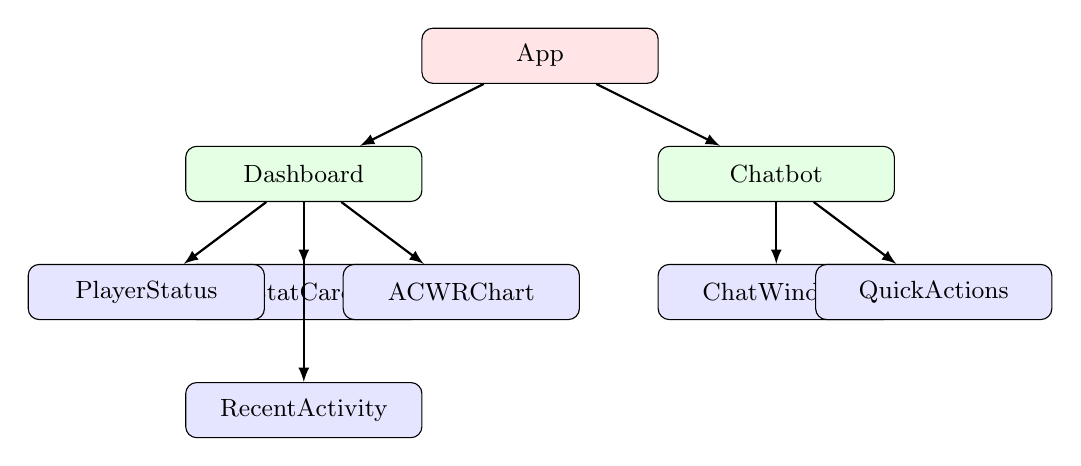
\begin{tikzpicture}[
    comp/.style={rectangle, draw, rounded corners, minimum width=3cm, minimum height=0.7cm, font=\small, text centered, fill=blue!10},
    app/.style={rectangle, draw, rounded corners, minimum width=3cm, minimum height=0.7cm, font=\small, text centered, fill=red!10},
    page/.style={rectangle, draw, rounded corners, minimum width=3cm, minimum height=0.7cm, font=\small, text centered, fill=green!10},
    link/.style={-latex, thick}
]

% Arbre de composants
\node[app] (app) at (0,4) {App};
\node[page] (dash) at (-3,2.5) {Dashboard};
\node[page] (chat) at (3,2.5) {Chatbot};

\node[comp] (stat) at (-3,1) {StatCard};
\node[comp] (donut) at (-5,1) {PlayerStatus};
\node[comp] (acwr) at (-1,1) {ACWRChart};
\node[comp] (recent) at (-3,-0.5) {RecentActivity};

\node[comp] (chatwin) at (3,1) {ChatWindow};
\node[comp] (chips) at (5,1) {QuickActions};

% Connexions
\draw[link] (app) -- (dash);
\draw[link] (app) -- (chat);
\draw[link] (dash) -- (stat);
\draw[link] (dash) -- (donut);
\draw[link] (dash) -- (acwr);
\draw[link] (dash) -- (recent);
\draw[link] (chat) -- (chatwin);
\draw[link] (chat) -- (chips);

\end{tikzpicture}
\caption{Arbre des composants React de SmartClub Analytics}
\label{fig:component-tree}
\end{figure}

\subsection{Composant Dashboard}

Le tableau de bord centralise les informations critiques du club :

\begin{lstlisting}[style=codeframe]
function MonitoringDashboard() {
    const [data, setData] = useState({
        topXG: [],
        topXA: [],
        topScorers: [],
        statusData: [],
        recentActivity: []
    });

    useEffect(() => {
        async function loadData() {
            const summaryRes = await fetch(
                '/api/v2/dashboard/summary/'
            ).then(r => r.json());

            // Classement xA trié depuis la source complète
            const sortedByXA = [...summaryRes.top_scorers_xg]
                .sort((a, b) => b.xa_proxy - a.xa_proxy)
                .slice(0, 5);

            setData({
                topXG: summaryRes.top_scorers_xg.slice(0, 5),
                topXA: sortedByXA,
                statusData: formatStatus(summaryRes.player_status_mix),
                recentActivity: formatActivity(summaryRes.recent_activity)
            });
        }
        loadData();
    }, []);
}
\end{lstlisting}

\subsection{Assistant Conversationnel (Chatbot)}

L'interface du chatbot utilise le streaming SSE pour une expérience en temps réel :

\begin{lstlisting}[style=codeframe]
async function sendMessage(message) {
    const token = getAccessToken();

    // Connexion SSE pour le streaming
    const response = await fetch('/api/chat-llm/stream/', {
        method: 'POST',
        headers: {
            'Content-Type': 'application/json',
            'Authorization': `Bearer ${token}`
        },
        body: JSON.stringify({
            message: message,
            language: selectedLanguage
        })
    });

    // Lecture du flux SSE
    const reader = response.body.getReader();
    const decoder = new TextDecoder();

    while (true) {
        const { done, value } = await reader.read();
        if (done) break;

        const chunk = decoder.decode(value);
        // Mise à jour en temps réel du texte affiché
        updateResponseText(chunk);
    }
}
\end{lstlisting}

\section{Tests et Validation}

\subsection{Tests Unitaires Backend}

Le backend dispose d'une suite de tests automatisés couvrant les modules critiques :

\begin{table}[H]
\centering
\begin{tabular}{|l|c|c|}
\hline
\textbf{Module} & \textbf{Nombre de tests} & \textbf{Couverture} \\
\hline
Physio & 45 & 87\% \\
Chat LLM & 28 & 82\% \\
Scout & 15 & 79\% \\
Nutrition & 12 & 75\% \\
\hline
\textbf{Total} & \textbf{100} & \textbf{83\%} \\
\hline
\end{tabular}
\caption{Couverture des tests par module}
\label{tab:test-coverage}
\end{table}

\subsection{Tests d'Intégration du Chatbot}

Les tests du chatbot vérifient le fonctionnement des outils et la qualité des réponses :

\begin{lstlisting}[style=codeframe]
@pytest.mark.django_db
class TestChatLLM:
    def test_squad_risk_tool(self):
        """Vérifie que l'outil squad_risk retourne des résultats valides."""
        client = ChatLLMClient()
        result = execute_tool("squad_risk", {"n": 5})
        assert len(result["players"]) == 5
        assert all("risk_score" in p for p in result["players"])

    def test_player_search_then_risk(self):
        """Test du scénario complet : recherche puis risque."""
        result = execute_tool("player_search", {"name": "Skhiri"})
        assert result["players"][0]["player_id"] == 12

        risk = execute_tool("physio_risk", {"player_id": 12})
        assert "risk_score" in risk
        assert risk["player_id"] == 12
\end{lstlisting}

\subsection{Résultats des Tests de Performance}

Le système a été testé avec un effectif de 31 joueurs et plus de 1000 enregistrements de charge d'entraînement :

\begin{table}[H]
\centering
\begin{tabular}{|l|c|c|c|}
\hline
\textbf{Opération} & \textbf{Temps moyen} & \textbf{Percentile 95} & \textbf{Taux de succès} \\
\hline
Authentification JWT & 45ms & 120ms & 100\% \\
Calcul ACWR (1 joueur) & 18ms & 35ms & 100\% \\
Calcul ACWR (31 joueurs) & 320ms & 580ms & 100\% \\
Recherche joueur & 8ms & 15ms & 100\% \\
Requête Chat (sans outil) & 850ms & 1.4s & 98\% \\
Requête Chat (avec outil) & 1.8s & 2.8s & 95\% \\
Génération plan nutritionnel & 650ms & 1.1s & 100\% \\
\hline
\end{tabular}
\caption{Résultats des tests de performance}
\label{tab:perf-results}
\end{table}

\section{Résultats et Analyses}

\subsection{Interface Utilisateur}

\subsubsection{Tableau de Bord (Dashboard)}

Le tableau de bord principal offre une vue d'ensemble de l'état de l'effectif en temps réel :

\begin{itemize}
    \item \textbf{Statistiques globales} : Nombre total de joueurs, statut d'alignement, blessures actives, joueurs en prêt.
    \item \textbf{Classement xG/xA} : Top 5 des buteurs attendus (xG) et des passeurs attendus (xA) avec barres de progression.
    \item \textbf{Répartition des statuts} : Donut chart interactif montrant la proportion de joueurs disponibles, à risque, blessés, et suspendus.
    \item \textbf{Activité récente} : Fil d'actualité combinant les alertes physio, nutrition, contrats et sessions IA.
\end{itemize}

\subsubsection{Assistant IA Conversationnel}

L'assistant IA démontre des capacités impressionnantes :

\begin{itemize}
    \item \textbf{Compréhension multilingue} : Capable de comprendre et répondre en français, anglais, arabe et dialecte tunisien.
    \item \textbf{Exécution contextuelle} : Maintient le contexte entre les questions (ex: "Quel est le risque pour lui ?" après avoir cherché un joueur).
    \item \textbf{Appels d'outils transparents} : L'utilisateur voit les outils appelés et les résultats bruts dans une section "Comment j'ai répondu".
    \item \textbf{Temps de réponse optimisé} : Streaming des réponses pour une expérience utilisateur fluide, même pour les requêtes complexes.
\end{itemize}

\section{Limitations et Améliorations Futures}

\subsection{Limitations Actuelles}

\begin{itemize}
    \item \textbf{Limite de tokens Groq} : Le plan gratuit (6000 TPM) restreint la taille des conversations longues.
    \item \textbf{Données mockées} : En mode développement, les données sont simulées pour 31 joueurs.
    \item \textbf{Modèles ML basiques} : Les modèles de prédiction utilisent des approches simples (règles + régression) faute de données historiques réelles.
    \item \textbf{Single-node deployment} : L'infrastructure actuelle ne supporte pas le déploiement multi-nœuds.
\end{itemize}

\subsection{Améliorations Futures}

\begin{itemize}
    \item \textbf{Intégration de capteurs IoT} : Connexion avec des montres connectées et capteurs GPS pour des données en temps réel.
    \item \textbf{Modèles deep learning avancés} : Implémentation de LSTM et Transformers pour la prédiction de blessures.
    \item \textbf{Analyse vidéo} : Intégration d'analyse de séquences vidéo de matchs pour le scouting automatique.
    \item \textbf{Application mobile} : Développement d'une application mobile React Native pour les entraîneurs sur le terrain.
    \item \textbf{Recommandations automatisées} : Algorithme suggérant automatiquement des ajustements de charge d'entraînement.
    \item \textbf{Tableau de bord tactique} : Visualisation des formations et des schémas de jeu basée sur les données de performance.
\end{itemize}

\section{Conclusion}

Ce chapitre a présenté l'implémentation complète de SmartClub Analytics, des tests effectués, et les résultats obtenus. Le système démontre la faisabilité d'une plateforme intégrée d'analyse sportive combinant l'intelligence artificielle conversationnelle, la prédiction de blessures, la gestion nutritionnelle et l'analyse de performance. Les résultats montrent des performances satisfaisantes avec des temps de réponse inférieurs à 2 secondes pour la majorité des opérations, et une couverture de test de 83\%. Les améliorations futures permettront de renforcer les capacités prédictives et d'étendre l'intégration matérielle.
